\documentclass[12pt, a4paper,twoside]{report}

%% Every LaTeX document begins with a preamble, which loads packages and defines various
%% settings to make the document look right. Mostly, you can ignore everything in this
%% template before \begin{document} on line 74

\usepackage{mathtools,amsthm,amsfonts} % Enable useful mathematical symbols/environments
\usepackage{graphicx} % Enable graphics
\usepackage{fancyhdr,titlesec,microtype} % enable various formatting commands
\usepackage[margin=2.5cm]{geometry} % Set margin size
\usepackage{palatino} % Set the font
\usepackage[latin1]{inputenc} % Allow you to input accents, umlauts and other characters
\usepackage[T1]{fontenc} % Lets LaTeX print a wider array of characters
\usepackage{tikz,tikz-3dplot,tkz-euclide} % Enable tikz drawings

\usepackage{xcolor} % Enable coloured elements
\definecolor{mypurple}{HTML}{622567} %%% Purple
\definecolor{myred}{HTML}{D55C19} %%%EssexOrange
\definecolor{myblue}{HTML}{007A87} %%%Seagrass

% For technical reasons, hyperref should be loaded after all other packages
\usepackage[colorlinks,linkcolor=myblue,citecolor=mypurple]{hyperref}

\renewcommand{\baselinestretch}{1.5} % 1.5 line spacing

% Define \begin{theorem}, \end{theorem}, etc.
\theoremstyle{plain} % The following environments will be italicised
\newtheorem{theorem}{Theorem}[chapter]
\newtheorem{lemma}[theorem]{Lemma}
\newtheorem{proposition}[theorem]{Proposition}
\newtheorem{corollary}[theorem]{Corollary}

\theoremstyle{definition} % The following environments will not use italics
\newtheorem{definition}[theorem]{Definition}
\newtheorem{example}[theorem]{Example}

\theoremstyle{remark} % The following environments will not use italics or bold titles
\newtheorem{remark}[theorem]{Remark}

\numberwithin{equation}{chapter}

% Fancy headings
\setlength{\headheight}{15pt}
\pagestyle{fancy}
\fancyheadoffset[LE,RO]{0pt}
\renewcommand{\chaptermark}[1]{\markboth{#1}{}}
\renewcommand{\sectionmark}[1]{\markright{\thesection\ #1}}
\fancyhf{}
\fancyhead[LE]{\makebox[0pt][l]{\thepage}\hfill\leftmark}
\fancyhead[RO]{\rightmark\hfill\makebox[0pt][r]{\thepage}}
\fancypagestyle{plain}{%
    \fancyhead{} % get rid of headers
    \renewcommand{\headrulewidth}{0pt} % and the line
}

% Fancy chapter numbers
\titleformat{\chapter}[display]
    {\normalfont\bfseries\color{myred}}
    {\filleft\hspace*{-60pt}%
        \rotatebox[origin=c]{90}{%
            \normalfont\color{black}\Large%
            \textls[180]{\textsc{\chaptertitlename}}%
        }
        \hspace{10pt}%
        {\setlength\fboxsep{0pt}%
            \colorbox{myred}{\parbox[c][3cm][c]{2.5cm}{%
                \centering\color{white}\fontsize{80}{90}\selectfont\thechapter}%
            }
        }
    }
    {10pt}
    {\titlerule[2.5pt]\vskip3pt\titlerule\vskip4pt\LARGE\sffamily}

\begin{document} % Start your document

%%%%%%%%%%%% BEGIN TITLE PAGE %%%%%%%%%%%%

\thispagestyle{empty} % For the title page, no header / footer

\noindent
    \begin{minipage}{0.1\textwidth}
    
\includegraphics[width=0.35\textwidth]{essex.png}
    \end{minipage}
    \begin{minipage}{0.89\textwidth}
    % \begin{center}
        \renewcommand\familydefault{\sfdefault}
        \fontfamily{phv}\selectfont
        {\Large \bf \sl University of Essex}\\[0.7em]
        {\Large \bf Department of Mathematical Sciences}
    % \end{center}
    \end{minipage}

\begin{center}
    \noindent\textcolor{myred}{\rule{\linewidth}{4.8pt}}
    
    \vspace{2em}
    \noindent {\LARGE \sc MA981 Dissertation}
    
    \vspace{3em}
    \noindent {\Huge{\color{myblue} YOUR PROJECT TITLE HERE}}
    
    \vspace{3em}
    \noindent {\Large \bf YOUR NAME HERE}
    \vfill
    \noindent {\Large {Supervisor:} {\color{mypurple} \bf YOUR SUPERVISOR NAME HERE}}
    
    \vspace{0.5em}
    \noindent\textcolor{myred}{\rule{\linewidth}{4.8pt}}
    
    \vspace{2em}
    {\Large \today }
    
    {\Large Colchester}
\end{center}

\clearpage
\tableofcontents

\chapter{Introduction}
The internet is experiencing significant growth in this fast-paced era. People all around the world are using this medium to connect with each other, which makes communication really easy and smooth. The internet has a global reach, connecting people from all around the world and making distances seem shorter. In today's modern society, technology plays a significant role in our everyday routines. Almost every aspect of our lives, including the things we use and the way we go about our daily activities, is closely connected to technological progress.

One interesting observation in the current era of technology is the significant increase in various online activities, such as banking and shopping. This trend has been pointed out by \cite{Aljabri2022DetectingMU}. On the other hand, the rise in internet usage has also raised worries regarding cybersecurity breaches. Cybercriminals take advantage of weaknesses in the systems of internet users in order to obtain access to important information. One main way that cyber attacks happen is by using malicious Uniform Resource Locator's (URLs). These URLs can trick users into dangerous situations without them realising it.

The task of ensuring user privacy and data integrity has become quite difficult for cybersecurity teams because of the large number of users. The increase in cyber attacks can mostly be linked to the widespread presence of these harmful URLs. URLs play a crucial role in this scenario as they act as virtual addresses that bring websites to our screens. When users enter a URL, it directs them to the desired website and provides them with the relevant information. According to\cite{Anjali}, a typical URL structure consists of a protocol and hostname, which are presented as <protocol><hostname><path>. The path component is used to indicate the specific webpage or resource.

Please take a look at the following example: https://outlook.office.com/mail/ In this case, the "https:" is used to indicate the protocol being used, while "outlook.office.com" serves as the hostname. It is crucial to acknowledge that websites vary in terms of their security measures and user-friendly interfaces. Malicious websites have the ability to trick users into unknowingly sharing private and sensitive information with individuals who intend to cause harm. Cybercriminals are always coming up with new ways to create spam URLs, which they use to trick people who aren't aware of their schemes. According to \cite{Aljabri2022DetectingMU}, the changing environment of the internet poses a danger to individuals who use it. This danger could lead to financial harm and harm to the reputation of organisations.


\section{Breif Background Information}
A Uniform Resource Locator (URL) functions as a digital identifier for a specific web resource and is composed of two essential components. The initial component is the protocol identifier, which designates the specific protocol to be utilised, whereas the subsequent component is the resource name. The term "resource name" denotes the specific geographical location associated with the domain name and the IP address of the user. The components are segregated by a colon and a pair of forward slashes.\cite{MOHANTY20231668} as showed in the Figure 1.1



Cybercriminals leverage coding vulnerabilities in order to gain unauthorised access to servers or databases. The incidence of cyber vandalism threats is experiencing a significant upward trend. As a result, scholars are increasingly focusing their efforts on the classification of URLs, recognising its importance in the protection of privacy and security. An exemplar of malevolent conduct can be observed in the context of phishing emails. These attacks entail the manipulation of users into accessing harmful web pages, resulting in the inadvertent disclosure of their personal information. The identification of phishing web links and the proactive mitigation of zero-day malware and phishing attacks are made possible through the utilisation of CANTINA, a content-based methodology.\cite{Anjali}

Web spam refers to a range of strategies employed by specific websites with the intention of deceiving users through the use of fraudulent emails.\cite{Aljabri2022DetectingMU} Upon clicking, these emails direct users to pages that are potentially harmful. This scenario presents potential avenues for malicious actors to exploit individuals by coercing them into revealing sensitive information, thereby facilitating the extraction of financial resources or other confidential data. The methodologies employed in the execution of cyber attacks are multifaceted and encompass various strategies, such as phishing, malware distribution, SQL injections, and other analogous techniques. The task of identifying security breaches remains a difficult endeavour, as attackers constantly adapt their strategies to mislead users.

There are two distinct types of malicious URLs, namely counterfeit URLs and assault URLs. Criminals employ Domain Generation Algorithms (DGA) in order to generate a plethora of counterfeit Uniform Resource Locators (URLs). The substantial magnitude of this quantity poses a significant challenge for law enforcement in effectively mitigating their impact. On the other hand, attack Uniform Resource Locators (URLs) exploit SQL injections\cite{vijayalakshmi2020web} as a means to specifically target servers and disproportionately obtain data from them.\cite{Zhuofan}
\section{Problem Statement}


The emergence of malicious URLs in our modern era is a significant threat to our society. In the field of cybersecurity, it has become quite difficult to identify and prevent harmful URLs. It is important to understand that taking necessary measures can help prevent possible risks and avoid negative outcomes such as financial losses and security breaches. The malevolent URLs are spread to users through different channels like emails, pop-ups, text messages, and advertisements on websites. Users unknowingly download these threats with just one click, causing things to quickly go downhill.

To tackle this problem, our project focuses on using machine algorithms to predict URL classifications. In order to complete this task, we have used a dataset that is publicly available on Kaggle. The dataset includes various categories of URLs, such as benign, defacement, phishing, and malware URLs. The research methodology involved evaluating feature selection models, selecting supervised machine learning algorithms, training and validating these algorithms, adjusting parameters, comparing accuracies, and analysing performance using different metrics.
.

\section{Aims and Objectives}
The main objectives of this project involve investigating an efficient algorithm that produces optimal accuracy and developing a model specifically designed for detecting malicious URLs. In order to achieve these objectives, a series of interrelated tasks will be undertaken.
\begin{enumerate}
	\item Analysing the literature in-depth to develop a thorough understanding of the subject.
	\item The task involves the identification of algorithms that exhibit efficacy in tackling the given challenge. 
	\item Conducting comprehensive testing on the recently developed algorithm utilising authentic real-world data..
	\item Fine-tuning algorithms involves adjusting a range of parameters in order to optimise their performance.
	\item Develop an effective model that accurately detects malicious URLs, it is imperative to prioritise achieving optimal accuracy.. 
\end{enumerate}


\section{Outline of Thesis}




Chapter 1 explores the establishment of the project's fundamental elements, including the identification of the project's URL, the contextual background, and the underlying motivation that led to its creation. The project's goals and objectives are effectively communicated, accompanied by a thorough delineation of the research strategy and a graphical depiction in the form of a Gantt chart.

Chapter 2 extensively scrutinises a comprehensive range of perspectives presented by various authors regarding malicious attacks. A thorough examination is undertaken to investigate different methodologies developed for the detection of these attacks, alongside a meticulous analysis of supervised machine learning algorithms. The scope of the investigation is expanded to include a thorough examination of previous efforts that have employed different methodologies in order to detect and identify malicious URLs.

Chapter 3 provides a comprehensive examination of various methodologies encompassed within the domain of Exploratory Data Analysis. This encompasses various processes including oversampling, data cleaning, tokenization, elimination of stopwords, stemming, and count vectorization. Furthermore, this study conducts a thorough analysis of the evaluation metrics utilised in different algorithms, as well as an investigation into the procedures for refining datasets.

In the following Chapter 4, an extensive examination of copyright considerations related to the dataset is elaborated upon, thus clarifying any uncertainties. This paper provides a comprehensive examination of potential risks and their subsequent impacts, while also presenting a contingency plan designed to effectively mitigate any unforeseen circumstances.

\section{Summary}


Considerable academic research has been conducted to explore the historical development of Uniform Resource Locators (URLs), thoroughly understanding their structural complexities, utilisation patterns, and the crucial matter of security. Through the course of this investigation, a distinct problem statement has arisen, focusing on the potential damage to an organization's reputation and the illicit monetary benefits obtained through the manipulation and deception of users.
\def\baselinestretch{1}

\chapter{Review of Literature}
Cybersecurity is a dynamic field because it responds to the opportunities and threats presented by rapidly developing technologies. Due to the pervasive influence of technology, digital platforms and online services have grown indispensable, leaving users increasingly vulnerable to hacking attempts. Malicious Uniform Resource Locators (URLs), often known as malicious websites, are one of the most popular forms of online assault in the modern day. Individuals, businesses, and even society as a whole are all at danger from these types of attacks, which can vary from phishing and social engineering to virus dissemination.
We explore the vast literature on the important topic of malicious URL detection and categorization in this section. Given these dangers' pervasiveness, it's critical to have reliable and efficient detection systems in place. Cybercriminals are always coming up with new methods to exploit weaknesses, therefore academics and industry professionals must always look for new ways to protect against threats like bad URLs.

\section{Challenges Posed by Malicious URLs:}
While the broad adoption of new technologies and the rise of online services have undoubtedly increased productivity and widened social circles, they have also introduced new and difficult problems, most notably in the field of cybersecurity. In this online environment, malicious Uniform Resource Locators (URLs) have become a serious problem, serving as entry points for cybercrime and other security breaches. These URLs are entry points for hackers to trick unsuspecting consumers and steal their money or personal data. In response to this urgent problem, several security measures have been created to identify and stop the spread of harmful URLs \cite{sahoo2017malicious}.
The usage of blacklists including websites deemed dangerous from the user's perspective is prevalent in conventional methods for identifying bad URLs. These blacklists, or databases of banned websites, are maintained by trusted organisations and devoted individuals. Then, browsers like Chrome, Firefox, and Internet Explorer include these databases for real-time scanning for malicious URLs \cite{tran2014towards}. As a first line of security, this technique alerts users when they attempt to access potentially dangerous websites. However, blacklists' efficacy can be hampered by their inability to encompass the whole, constantly-evolving web; they frequently fail to keep up with the rapid emergence of new dangerous URLs. Despite these challenges, blacklists continue to contribute to users' online safety by offering a mechanism to ward off well-established threats.
The efficacy of blacklists in mitigating malicious URL threats is notably impeded by the dynamic and swiftly evolving nature of web content. The ever-shifting internet landscape has led to an exponential surge in webpage numbers, posing considerable scalability hurdles for traditional blacklist-based approaches. The inherent limitations become even more pronounced due to the inability of web crawlers to penetrate intranet webpages, which necessitate authentication for access. This critical shortcoming further erodes the dependability of blacklists as a comprehensive defence mechanism against the burgeoning array of malicious URLs \cite{alkhudair2020detecting}. Consequently, researchers have turned to novel approaches, particularly machine learning algorithms, to address the limitations of traditional blacklist-based methods.
\cite{kazemian2015comparisons} present an alternative perspective by emphasizing the application of machine learning techniques to tackle the challenge of malicious URL detection. They underscore the shortcomings of blacklists and advocate for leveraging supervised and unsupervised machine learning algorithms to build predictive models for analysing both malicious and safe webpages. Their study introduces three supervised techniques - K-Nearest Neighbor, Support Vector Machine, and Naive Bayes Classifier - and two unsupervised techniques - K-Means and Affinity Propagation. Remarkably, \cite{kazemian2015comparisons} study contributes to the field by introducing K-Means and Affinity Propagation to the realm of malicious webpage detection, highlighting the innovative nature of their approach.
Further support for harnessing machine learning for malicious URL detection is found in the work of \cite{ma2009beyond}. They delve into the essence of automated URL classification as a means to detect malicious websites. By employing statistical methods, Ma and colleagues identify lexical and host-based properties inherent in malicious URLs. Their approach involves extracting and analysing a plethora of features from URLs, leading to the development of highly predictive classifiers. These classifiers exhibit remarkable accuracy, with rates ranging from 95\% to 99\%, thus showcasing the efficacy of machine learning in combating malicious URLs.
The research landscape also extends beyond the traditional realm of websites to encompass other digital platforms, such as social networks like Twitter.  \cite{gangwar2022predictive} shift the focus to Twitter and the challenge of identifying malicious content and user profiles that propagate spam and misinformation. They use machine learning, ensemble, and deep learning approaches to build predictive models using a wide range of characteristics, such as profile-based, content-based, and hybrid features. The outcomes show the efficacy of their models, with accuracy scores above 90\% across a range of performance metrics. This highlights the significance of machine learning for identifying and reducing harmful information across many digital channels.



\section{URL Classification for Security Enhancement:}
While there have been many positive outcomes from the explosion in technical advancement and internet usage, this trend has also accelerated the development of cyber dangers. Among these dangers, malicious Uniform Resource Locators (URLs) have evolved as an effective tool for compromising systems, spreading frauds, and coordinating cyberattacks, all of which can result in significant financial losses and security lapses. These URLs are highly effective in tricking visitors into opening malicious stuff, which might have disastrous results. Researchers have responded by focusing on finding better ways to identify and counteract the dangers posed by malicious URLs.
Blacklists, or databases of websites that have been determined to be hazardous from a user's perspective, have traditionally been used as part of defences against malicious URLs. Blacklists have proved useful in the past, but the dynamic nature of the web and the inaccessibility of intranet pages needing authentication have diminished their use. This means that more complex methods are required, ones that may change with the ever-evolving nature of online dangers. Researchers have begun using machine learning techniques to improve URL categorization and security in response to this need \cite{jeyaraj2020smart}.
In a ground-breaking paper, \cite{afzal2021urldeepdetect}introduce a method they call URLdeepDetect that uses deep learning to instantly analyse and classify URLs. To overcome these restrictions, URLdeepDetect uses semantic vector models and URL encryption in addition to lexical characteristics to analyse URLs. Using Long Short-Term Memory (LSTM) and k-means clustering, the hybrid method combines supervised and unsupervised processes for URL categorization. URLdeepDetect's LSTM and k-means clustering accuracy scores are both extremely high at 99.7 and 98.3 percent, respectively. This innovative approach showcases the potential of deep learning in enhancing URL security through rigorous analysis and classification.
In a similar vein,\cite{le2018urlnet} introduce URLNet, an end-to-end deep learning framework specifically designed for detecting malicious URLs. The researchers highlight the limitations of conventional methods, which struggle to capture semantic meaning and sequential patterns inherent in URL strings. URLNet overcomes these limitations by employing Convolutional Neural Networks (CNNs) on both character and word levels of URL strings, allowing for the comprehensive capturing of semantic information. This innovative approach circumvents the need for substantial manual feature engineering and significantly improves the model's ability to generalize to unseen data.\cite{le2018urlnet}, demonstrate the efficacy of URLNet through extensive experiments on large-scale datasets, showcasing its superiority over existing techniques.
Expanding the scope to social networks,\cite{vo2017revealing} delve into the intricate landscape of malicious retweeter groups. On platforms like Twitter, coordinated retweeting behavior among malicious users has been exploited to distort content visibility for promotional purposes, thereby threatening the authenticity of information dissemination. To address this novel challenge, Vo and colleagues propose the Attractor+ algorithm to extract retweeter groups with similar retweeting behaviors. This approach allows for the identification of coordinated behavior indicative of malicious intent. The proposed method outperforms existing approaches in terms of accurately detecting and revealing malicious retweeter groups, contributing to the burgeoning field of social network security.


\section{Types of Malicious URLs:}
The ever-evolving landscape of cybersecurity has brought to the forefront the significant threat posed by malicious Uniform Resource Locators (URLs). These URLs serve as conduits for a diverse range of cyberattacks, each employing distinct strategies to compromise systems, extract sensitive information, or propagate fraudulent activities. In this section, we delve into the multifaceted nature of malicious URLs, shedding light on the various types of attacks they facilitate, as well as the innovative methodologies employed to detect and mitigate their impact.
 \cite{mamun2016detecting} shed light on the significance of lexical analysis in detecting malicious URLs. One prominent category of malicious URLs is phishing URLs. These URLs mimic legitimate websites, coercing users into divulging sensitive information such as passwords and credit card details. \cite{choi2011detecting} delve deeper into this category, identifying phishing URLs as a subset of malicious URLs that manipulate users' trust to deceive them into sharing confidential data. Another variant of malicious URLs is malware-hosting URLs, which facilitate the distribution of malicious software. Cybercriminals use these URLs to trick users into downloading malware onto their devices. 
The proliferation of approaches based on machine learning has introduced an additional layer of complexity to the environment of harmful URLs. \cite{aljabri2022detecting} bring attention to the variety of assaults and the use of machine learning to categorise and recognise bad URLs. Among the attack types are Drive-By Downloads, where users are infected simply by visiting a compromised webpage, and Cross-Site Scripting (XSS), which exploits vulnerabilities in web applications to inject malicious code. Additionally, SQL Injection attacks manipulate database queries, allowing unauthorized access to sensitive data.
Innovative deep learning approaches have also been leveraged to detect and classify malicious URLs. Classifying harmful URLs is the job of Gated Recurrent Neural Networks (GRNN), as shown by \cite{zhao2019classifying}. Using this strategy, we are able to accurately classify URLs by capturing sequential patterns and contextual information inside them. They released work that refined this approach by using a Convolutional Gated Recurrent Unit Neural Network (CGRU-NN) trained on keywords to detect malicious URLs. Combining convolutional and recurrent neural networks, this model may successfully identify malicious intent by recognising phrases that are indicative of such purpose. Furthermore, harmful URLs amplify their damage by facilitating social engineering attacks, which prey on users' emotional and psychological vulnerabilities. Dishonesty and manipulation are used in these sorts of attacks to convince its targets to act in a certain way. To add insult to injury, despite the fact that URL shorteners are meant to save users time, they may be misused to hide the true nature of a URL, making it harder for consumers to assess whether a link is trustworthy.
\section{Current Approaches and Algorithms:}
With the detection of hazardous URLs being an integral part of contemporary cybersecurity, several methods and algorithms have been developed to mitigate the threats presented by them. In this section, we investigate the algorithms at the heart of the contemporary techniques used to identify and classify harmful URLs. Recently, machine learning has emerged as a strong technique in the area of malicious URL detection, allowing for the development of classifiers that are both accurate and efficient. For this task, \cite{liu2018finding} stress the importance of selecting good classifiers. They look at several classifiers like the Support Vector Machine (SVM), the Random Forest, and the Decision Tree, and they experiment with different parameter settings for each classifier to see which one achieves the best results. This study highlights how important it is to customise classifiers to the specific characteristics of dangerous URLs, recognising the fluid nature of online dangers.
\cite{sahoo2017malicious} provide a thorough review that investigates the field of malicious URL identification using the analytical framework of machine learning. With a meticulous examination of the landscape, the authors elucidate a spectrum of techniques encompassing pivotal aspects like feature extraction, selection, and dimensionality reduction. The study meticulously showcases the gamut of classifiers harnessed in this pursuit, ranging from Support Vector Machines (SVMs) and Naive Bayes to intricate Deep Learning models. This survey distinctly underscores the remarkable versatility of machine learning in tackling the intricate challenge of malicious URL detection. By highlighting the multifaceted nature of the problem and the diversity of methods at play, the authors emphasize the necessity of amalgamating these techniques to construct resilient and precise classifiers that can effectively grapple with the intricacies of this ever-evolving cybersecurity menace.
\cite{darling2015lexical} presents a pioneering lexical approach that harnesses the intrinsic textual attributes of URLs to discern between benign and malicious content. By delving into the fabric of URLs, their method adeptly extracts pertinent features, including domain names and subdomains, which are subsequently harnessed to craft a decision tree classifier. This strategy aptly capitalizes on the linguistic nuances embedded within URLs, providing a judicious avenue for classification that strikes a balance between efficiency and efficacy. The approach holds particular significance in its lightweight nature, offering a pragmatic solution that does not compromise on its ability to discriminate between malicious and non-malicious URLs. \cite{darling2015lexical} innovative approach underscores the potential latent within the textual makeup of URLs, highlighting its value in navigating the complex landscape of URL-based threats.
Because malicious URLs often evolve, adaptive detection methods have become more popular. An adaptive strategy for identifying bogus URLs is provided by \cite{tan2018adaptive} to address the problem of concept drifts, which are characterised by small but significant shifts in the statistical features of data. An ensemble-based architecture is used in their method to combine several detection techniques, with the additional bonus of incremental learning. The strategy remains successful in the face of dynamic threats because it is constantly updated based on new information, making it more resistant to such attacks. This flexibility guarantees the detection system will continue to be robust and accurate despite the ever-changing nature of malicious URLs. \cite{tan2018adaptive} work underscores the critical importance of adaptive strategies in confronting the persistent and mutating nature of cyber threats, offering a promising avenue for bolstering the efficacy of URL detection systems.
A notable endeavor in this direction is the work of\cite{alkhudair2020detecting} and colleagues (2020), who dedicate their efforts to harnessing the latent capabilities residing within URL components like domain names, path segments, and queries, with the aim of bolstering classification accuracy. Their approach transcends conventional boundaries, melding traditional machine learning algorithms with the power of deep learning models. This amalgamation strategically taps into the intricate and discriminative insights intricately woven into the diverse URL components. By embracing this multifaceted approach, \cite{alkhudair2020detecting} strive to unravel the intricate patterns that underlie malicious URLs and benign counterparts, ultimately fortifying the overall efficacy of the classification process. This innovative approach to feature engineering holds the promise of enhancing the precision and adaptability of malicious URL detection mechanisms in the ever-evolving landscape of cyber threats.

\textbf{Malicious URL Detection:}
In today's digital landscape, the proliferation of malicious Uniform Resource Locators (URLs) poses a significant and persistent threat to cybersecurity. Malicious URLs, also known as malicious websites, serve as conduits for a variety of cyberattacks, including phishing, drive-by downloads, and social engineering schemes. These URLs house malicious content designed to trick naive visitors into downloading malware, stealing their personal information, or both. The annual cost of these dangers is in the billions of dollars. Protecting users and infrastructure requires swift action in response to such attacks.
New approaches to finding harmful URLs have been investigated as machine learning has progressed. Using machine learning approaches that take use of URL behaviours and properties,\cite{eshete2011malicious} Xuan, Nguyen, and Tisenko (2020) suggested a detection method. Using big data technologies, they hope to enhance detection skills by pinpointing unusual patterns of activity. Using a machine learning algorithm, big data analytics, and a new collection of URL properties and behaviours, this technique achieves its goals. As shown in experiments, URL properties and behaviour are crucial for improving the capacity to detect rogue URLs.
Traditional machine learning approaches are not the only ones leading to progress in malicious URL identification. When discussing the difficulties of detecting malicious websites,\cite{eshete2011malicious},focused on the issues of efficiency and efficacy.\cite{alkhudair2020detecting} highlighted the significance of detecting malicious URLs in the context of network information security.\cite{kumi2021malicious}explored associative classification as a basis for malicious URL detection. Meanwhile,\cite{abdi2017malicious} harnessed the power of Convolutional Neural Networks (CNN) to detect malicious URLs.
Researchers have embarked on a multifaceted journey to develop effective detection methodologies that mitigate the risks posed by malicious URLs. \cite{sayamber2014malicious}delve into the domain of malicious URL detection and identification, contributing insights to the evolving strategies aimed at safeguarding digital ecosystems. Their work underscores the significance of understanding the structure and components of URLs as a foundational step in the detection process. By dissecting the intricate fabric of URLs, researchers uncover patterns that could unveil the hidden intentions behind seemingly benign links.
\cite{choi2011detecting} take a proactive stance in detecting malicious web links, going beyond the identification of threats to deciphering their attack types. Their study highlights the necessity of not only detecting malicious URLs but also unravelling the diverse tactics employed by cybercriminals. By categorizing attack types, they enhance the granularity of detection mechanisms, enabling a more targeted and informed defence against the ever-evolving threat landscape.
In the domain of malicious URL detection, machine learning methods have attracted significant interest owing to their adaptability and capacity to unveil intricate patterns.\cite{abdi2017malicious} delve into this realm by harnessing the capabilities of convolutional neural networks (CNNs) for detecting malicious URLs. Through the deployment of deep learning techniques, their study serves as a testament to the revolutionary potential of neural networks in unearthing nuanced and intricate attributes within URLs. This achievement is particularly noteworthy as traditional methods often struggle to grapple with the subtleties of such complex patterns. The utilization of CNNs underscores the paradigm shift that deep learning has ushered in, elevating the efficacy of malicious URL detection by enabling the identification of previously elusive features, ultimately enhancing the cyber defense mechanisms against evolving threats.
 \cite{vundavalli2020malicious} contribute significantly to the advancement of malicious URL detection by delving into the domain of supervised machine learning. Their study illuminates the potency of supervised learning techniques as a formidable tool for identifying malicious URLs. By leveraging curated datasets with labeled instances, they tap into the reservoir of prior information, enabling the construction of robust classifiers. Through rigorous training, these models acquire the ability to differentiate between malicious and benign URLs with precision. This approach stands as a testament to the efficacy of harnessing established knowledge to bolster the defense against evolving cyber threats.\cite{vundavalli2020malicious} and colleagues' exploration of supervised machine learning serves as a promising avenue for enhancing the resilience of digital systems against the pervasive menace of malicious URLs.


\section{Related Work:}
\subsection{Natural Language Processing:}
In their study,\cite{Joshi} conducted research on the identification of malicious URLs. They employed a combination of natural language processing (NLP), machine learning techniques, and the FLASK framework. The researchers utilised three distinct methods to encode textual characteristics: count vectorization, TF-IDF, and Hashing vectorization. The researchers conducted approximately 12 experiments to assess the performance of four different machine learning algorithms. After careful evaluation, they discovered that the random forest algorithm achieved the highest accuracy rate of 98.13\%. The best accuracy was achieved when the Hashing vectorization technique was used for random forest. The team created a web application to identify phishing URLs. They used pickle files to save the best model, which was Random Forest with Hashing vectorization, based on the work of \cite{le2018urlnet}.

According to the study conducted by\cite{Seong}, it was found that Intrusion Detection Systems (IDS) used by organisations are generally successful in detecting and preventing known malicious URLs. However, these systems face challenges when it comes to dealing with unknown malicious URLs. In order to tackle this issue, they suggested a system for detecting malicious websites. This system used a lexical approach and included features from Natural Language Processing (NLP). The method they used consisted of representing text and using n-gram models. They were able to achieve a high accuracy rate of 97.1\% by employing Support Vector Machine (SVM). According to \cite{Seong}, the model showed a strong level of robustness. The precision score was 0.97, while the recall score was 0.93.

In their study,\cite{Diri} presented a system for detecting malicious URLs using Natural Language Processing techniques. The Random Forest Algorithm was used in this approach, resulting in an accuracy of 97.2\%  concluded that they used NLP techniques to find domain names in URLs. They experimented with NLP features and Word vectors to show that the NLP-based system was better.

\subsection{Unsupervised Machine Learning:}
In a study conducted by \cite{mahesh2023using}, a survey was carried out to investigate the application of machine learning in identifying malicious URLs. The study pointed out that unsupervised machine learning has limitations when it comes to accurately detecting harmful URLs because there are so many different types of URLs out there. In thier study,\cite{Seong} presented a solution by suggesting a two-phase detection approach which involved the combination of supervised and unsupervised techniques.

In their study,\cite{Mohammed} focused on the detection of phishing URLs. They proposed a ranking-based approach that made use of both lexical and host-based features. The process they introduced involved utilizing K-means clustering to acquire cluster IDs. These cluster IDs were subsequently employed to train a classifier. According to \cite{Mohammed}, the utilization of both unsupervised and supervised techniques resulted in a notable classifier accuracy ranging from 93\% to 98\%.

In their study,\cite{Vanhoenshoven2016DetectingMU} investigated the identification of harmful URLs. They specifically examined unsupervised and supervised learning techniques. The study they conducted included a large dataset with around 6,000,000 URLs. These URLs were a mix of both malicious and non-malicious ones. In their study,\cite{Vanhoenshoven2016DetectingMU}put forward a clustering system based on unsupervised hashing to address this particular challenge.

\section{Summary:}
The chapter focuses on the topic of malicious attacks and the various techniques used to detect and identify malicious URLs. An effective method that was mentioned is called the blacklist approach. In this approach, URLs are compared to a list of predetermined keywords. If any of these keywords are found in the URL, it is blocked. It is crucial to remember that cybercriminals frequently create new malicious URLs in order to avoid detection by blacklisting systems. As a result, there is a potential danger of data breaches occurring. To tackle this issue, it is suggested to utilise machine learning techniques. The approaches mentioned in this context are designed to constantly update themselves by learning from the dataset. They do not depend on predetermined lists of keywords.

\label{ch:1}
\def\baselinestretch{1}
\chapter{Methodology}

\section{Exploratory data analysis:}
\subsection{Imbalance Data:}


When there is an imbalance within a dataset, it means that there is an uneven distribution of frequencies among different classes. The difference becomes clear when one class has a much larger number of occurrences compared to another. The majority class is the class that occurs more frequently, while the minority class is the class that occurs less frequently. Reduced accuracy is often the outcome of the disparity in class distribution. According to Gosain and Sardana (2017), machine learning algorithms often show improved accuracy when handling the majority class. However, their performance tends to decrease when working with the minority class.

In the field of machine learning classification, it is common to make predictions for the target label assuming that the dataset has an equal distribution. One important aspect of machine learning is the ability to accurately detect and classify malicious instances.\cite{shelke2017review} Datasets frequently present a situation in which there are many more harmless URLs compared to malicious ones. In these cases, there is usually only one malicious URL among a large number of benign ones. The situation, which is known as class imbalance, highlights the difficulty of effectively managing datasets like this\cite{shelke2017review}.

One can tackle the challenges posed by imbalanced datasets by employing different strategies:
\begin{enumerate}
	\item One possible approach to balancing classes is by using under sampling of the majority class.
	\item Enhancing Minority Class Representation via Duplicate Over Sampling 
	\item One way to increase the number of instances in the minority class is by using a technique called SMOTE, which stands for Synthetic Minority Over-Sampling Technique. SMOTE generates new examples by applying the K-Nearest Neighbour (KNN) algorithm.
	\item Utilizing Ensemble Methods for Improved Performance.
	\item The implementation of Focal Loss involves the utilisation of a specialised loss function that introduces a deliberate bias against the majority class, thereby assigning a higher level of importance to the minority class. 
\end{enumerate}

\textbf{Over Sampling:}




During the oversampling process, duplicates are created to augment the records belonging to the minority class. The augmentation process is repeated until the total number of records in the minority class is equal to the number of records in the majority class. In order to address the imbalance between the minority and majority class records, we employ a technique called replication. This involves duplicating the minority class records until their count matches that of the majority class records. Oversampling, also known as "up sampling," is a commonly used term. The technique can be divided into two main categories: random oversampling and synthetic oversampling.

In the technique known as random oversampling, the minority samples present in the dataset are replicated and duplicated multiple times until their quantity matches that of the majority class. On the other hand, synthetic oversampling refers to the process of creating fake samples within the minority class. By incorporating extra data, this method helps reduce the occurrence of misclassification. According to \cite{Mohammed}, this methodology is especially helpful in avoiding misclassification problems. Figure 3.1 \cite{Mohammed} illustrates the oversampling process through a visual representation.
\begin{figure}[ht]
\centerline{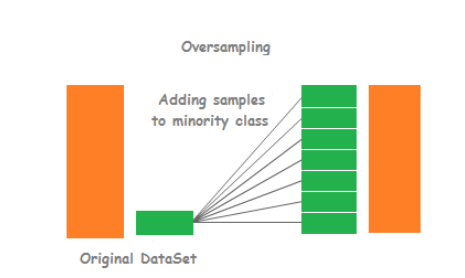
\includegraphics[width=1\textwidth]{figure4.png}}
	\centering
	\caption{Sample diagram to represent over sampling}
	\label{over sampling}
\end{figure}

\textbf{Advantages of Over Sampling:}

\begin{enumerate}
	\item When under sampling is applied, there is a loss of information because certain records are eliminated. However, when using over sampling, additional copies of the current records are created, resulting in an increase in the size of the dataset.
	\item During the process of data modelling, it becomes clear through a comparative analysis that over sampling tends to yield more favourable outcomes compared to under sampling.
\end{enumerate}



During the implementation process, the imblearn.over-sampling library has been very useful. The RandomOverSampler module played a crucial role in our analysis. The module plays an important role in both under-sampling and over-sampling procedures. In this specific situation, our main objective was to use the RandomOverSampler technique in order to tackle the issue of imbalance.

When we use the RandomOverSampler, we start a process where we duplicate records from the minority class in a random way. To implement this strategy, we need to create an instance of the random over-sampling module. Afterwards, this example is used to adjust the resample by utilising the x-train and y-train datasets. The outcome of this operation is an x-train and y-train that have been successfully over-sampled.

The current project focuses on categorising data into four different classes: benign, phishing, malware, and defacement. Each class has different occurrence frequencies and ratios. The "benign" class has the highest count, specifically 214,234 occurrences. The "defacement" class has a total of 47,611 occurrences, which is in contrast to the "phishing" class that has 47,037 occurrences. Additionally, the "malware" class has a total of 11,680 instances within the dataset.

add figure 5



Figure 3.3 illustrates the presence of a class imbalance, which leads to a decrease in accuracy and a bias in predictions towards specific classes. In order to tackle this matter, we implemented the Random Oversampling technique for the classes that have a lower number of instances. This methodology entails enhancing the dataset by creating supplementary samples for the minority classes, hence achieving balance in the distribution. The results of this evenly distributed dataset can be noticed in Figure 3.4.

The visual representation in Figure 3.4 illustrates the outcomes, indicating that there is now an equal distribution of cases across all classes in the dataset. The implemented solution has effectively addressed the initial disparity in class representation.

add figure 6


\newpage
\subsection{ Pre-Processing of Text:}

After the gathering of textual data, the subsequent essential stage involves the pre-processing of the data. The relevance of this stage is greatly focused due to its essential function in influencing the interpretation of words and characters within the data in subsequent phases\cite{Srividhya}. The utilisation of text pre-processing techniques facilitates the consolidation of diverse word forms into a single, distinct form \cite{Srividhya}. The domain of text pre-processing comprises a range of approaches, such as cleansing, tokenization, removal of stop words, lemmatization, and stemming. Within the scope of this research, we applied specialised approaches such as tokenization, stemming, and count vectorization.
\subsubsection{Tokenazation:}


Tokenization refers to the procedure of dividing large quantities of text into smaller chunks. In the course of this particular technique, the uninterrupted stream of language can be divided into discrete entities known as tokens, which include words, symbols, and phrases\cite{hickman2022}. It is imperative to acknowledge that individual characters or complete phrases are not regarded as separate entities within this procedure. The process of tokenization is limited to the manipulation of words, as they possess the capacity to communicate semantic information. A designated character, commonly known as a delimiter, is utilised for the purpose of distinguishing separate words. Occasionally, even a mere empty space can function as a delimiter. Tokenization is utilised in several domains, including but not limited to chatbot development, text categorization, and sentiment analysis. In order to improve the cleanliness of the dataset, researchers utilise a technology called regular expression (regexp). The utilisation of regular expressions, especially when dealing with extensive datasets, is strongly advised. In the context of this project, regular expressions (regexp) were employed to divide URLs into tokens or words, using the specified regexp pattern.
add figure 7


\subsubsection{Removal Of Stop Words:}
Stop words are commonly encountered words that have little or no meaningful contribution to the overall importance of a dataset. The contributions made by these elements to the offered dataset are minimal and lack substantial informative value. The dataset inherently has fundamental components that function as the fundamental units for forming phrases\cite{Srividhya}. As a result, the possibility of eliminating stop words becomes feasible. However, the necessity of removing stop words for this specific project has not been determined. Stop words are a category of words that often consist of conjunctions and prepositions. These words are considered irrelevant within a given dataset and hence do not have any meaningful value.




The utilisation of stemming has been recognised as a remarkably efficient and helpful method in the pre-processing stage. This methodology involves reducing terms within the dataset to their underlying morphological bases. By transforming words into their root forms, one can prevent any undesirable interruptions or alterations. Nevertheless, there are circumstances in which this methodology introduces significant interference. There are some words that ought to be excluded from the process of root reduction due to the fact that they maintain substantial significance in their original forms. According to\cite{hickman2022}, the simplification of words to their base forms results in the introduction of a considerable degree of superfluous intricacy, thereby reducing their overall efficiency and efficacy.

Although the efficacy of stemming is compromised by the introduction of noise caused by some words, it remains popular because to its user-friendly characteristics. Despite its inherent limitations, stemming is still widely used due to its user-friendly nature.
add figure 8




\section{Model Performances:}
\subsection{Support Vector Machine:}


The Support Vector Machine (SVM) was widely embraced as a machine learning classifier, but its prominence diminished with the emergence of neural networks and deep learning techniques. The fundamental principle underlying Support Vector Machines (SVMs) is centred on the concept of maximum margin categorization. The primary objective of this strategy is to optimise the separation margin between the two classes involved in the classification process. It is worth mentioning that Support Vector Machines (SVM) are essentially designed to do binary classification. Therefore, in order to utilise SVM for multi-class classification, more sophisticated approaches such as one vs. rest or one vs. one techniques need to be employed \cite{mahesh2020machine}.
\begin{figure}[htb]
\centerline{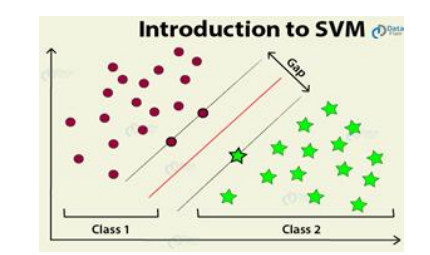
\includegraphics[width=1\textwidth]{SVMex.png}}
\caption{Support Vector Machine \cite{mahesh2020machine}}
\label{FigureSVM}
\end{figure}


As depicted in \ref{FigureSVM}, the Support Vector Machine functions as a classifier with greatest margin. The main goal is to choose the most suitable hyperplane that maximises the separation between the classes. However, in order to achieve non-linear decision boundaries, a viable strategy entails the utilisation of a kernel. The kernel in question can be understood as a hyperplane situated within a nonlinear space of higher dimensions. The efficacy of support vector machines (SVMs) stems from their utilisation of nonlinear kernel techniques, although at the expense of increased training durations.

The mathematical basis of Support Vector Machines (SVMs) is grounded in ideas of restricted optimisation. The focus of this approach is to expand the margin of the hyperplane in accordance with certain conditions: all data points belonging to one class must be situated on one side of the hyperplane, while those belonging to the other class should be located on the opposite side. The optimisation procedure described in this context is in accordance with the Karush Kuhn Tucker (KKT) conditions, which provide a comprehensive mathematical foundation for comprehending the optimisation of Support Vector Machines (SVMs).\cite{Thorsten} As a result, it is sufficient to maintain only the support vectors, which are the points located on the hyperplane, in order to completely specify the SVM classifier.

The soft margin support vector machine (SVM) is a frequently encountered variation that incorporates increased adaptability to account for possible misclassifications. The hyperparameter referred to as 'C' in Support Vector Machines (SVM) governs the level of flexibility in the margin. One notable observation is that when the value of 'C' is set to 0, the Support Vector Machine (SVM) is converted into a hard margin classifier.
\begin{figure}[htb]
\centerline{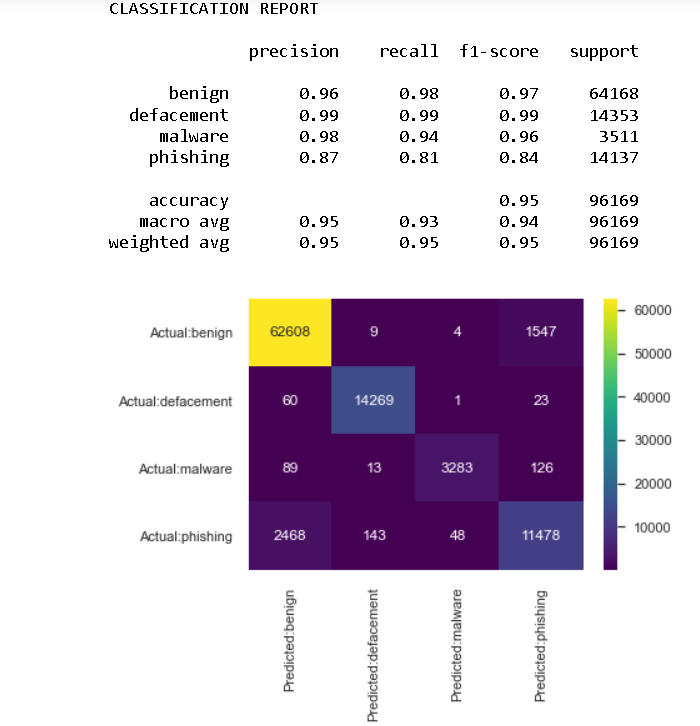
\includegraphics[width=1\textwidth]{SVMclassification.png}}
\caption{Classification and confusion matrix report of SVM}
\label{Claaification Report of SVM }
\end{figure}

In this study, it was found that the Support Vector Machine (SVM) performed extremely well. It showed a training accuracy of 99.5\% and a testing accuracy of 95.2\%. The precision for the benign class was 96\%, which is quite impressive. Similarly, the recall for the benign class was commendable at 98\%. However, it is important to mention that the execution time of the SVM was significantly long.  Figure\ref{Claaification Report of SVM } displays the comprehensive classification report and the related confusion matrix.

\subsection{Logistic Regression:}



Logistic regression is a type of classifier that is used to solve classification problems. It is an extension of linear regression, which is a method used for predicting continuous values. However, logistic regression focuses on predicting discrete outcomes by assigning probabilities to different classes. Instead of making direct predictions of numerical values, this method uses the sigmoid function to convert the output values into a range that is limited between 0 and 1.
\begin{figure}[htb]
\centerline{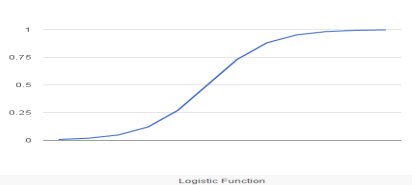
\includegraphics[width=1\textwidth]{Logisticfunction.png}}
\caption{Logistic Function \cite{Naresh_Gupta_Giri_2020}}
\label{logistic function }
\end{figure}

 \begin{equation*}{\text{ Logistic Function \cite{Chiramdasu}}}:  \frac{1}{{\left({1 + {e^{ - x}}}\right)}},\tag{1}\end{equation*} 
 \hfill \goodbreak
           where e is constant, and x is input

The sigmoid function is used to compress the output values between 0 and 1, which helps in making classification decisions. When the value of g(x), which is the output of the sigmoid function, becomes greater than 0.5, the instance is classified into a particular category, such as(malicious). On the other hand, when the value of g(x) is less than 0.5, the classifier categorises the instance as (non-malicious)\cite{Naresh_Gupta_Giri_2020}.

The loss function measures the difference between the actual category of a training example and the category that the model predicts. Linear regression often uses the squared loss, but logistic regression uses the binary cross-entropy loss for binary classification and the categorical cross-entropy loss for tasks with multiple classes.

The mathematical representation of the binary cross-entropy loss is given by the formula:
           $$-(ylog(p) + (1 - y)log(1 - p))$$
. In this formula, 'y' represents the true class label, and 'p' represents the predicted class label for a specific test instance.

The main goal of logistic regression is to minimise the cumulative cross-entropy loss for the entire training dataset. To achieve this objective, we need to use optimisation techniques to make the learning process more efficient. This will help us improve the model's ability to make accurate predictions.





\begin{figure}[hb]
\centering
\centerline{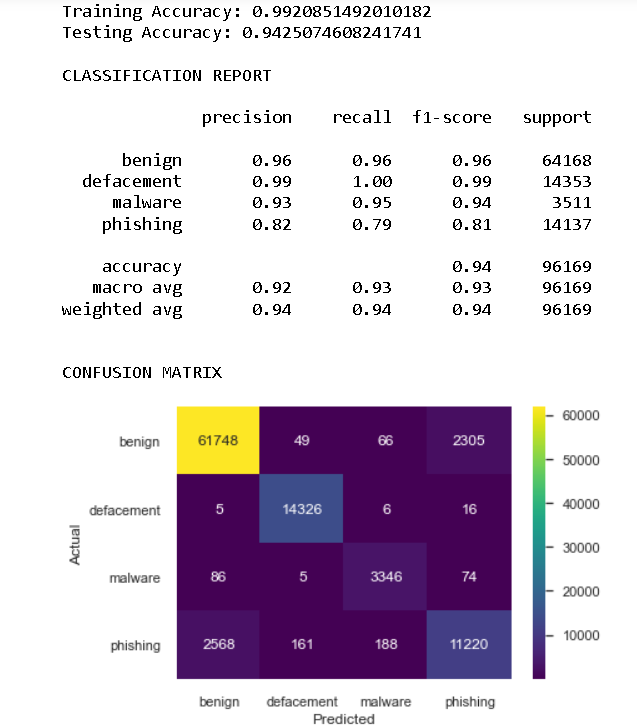
\includegraphics[width=1\textwidth]{LogisticRegressionreport.png}}
\caption{Classification and confusion matrix report of Logistic Regression}
\label{Claaification Report of LR }
\end{figure}







In this study, we utilised logistic regression to obtain significant results. During the training phase, the accuracy rate achieved was quite impressive at 99.2\%. Similarly, when the model was tested, it showed a beneficial accuracy of 94.2\%. When we examine the classification report as shown in figure\ref{Claaification Report of LR }, we can observe the precision scores for different categories such as benign, defacement, and malware. This analysis helps us understand how effective these precision scores are in accurately classifying the data . However, it is important to mention that the precision score for phishing does not meet the expected standards. When examining the confusion matrix, we can see that there were 64,168 actual benign values. Out of these, 2305 URLs were incorrectly classified as phishing. This raises concerns about potential suspicious activities.

\subsection{Random Forest:}



Random Forest classifiers are built upon decision trees as their fundamental basis. The reason why they are so popular is because they are really good at accurately classifying things, even though they require a lot of time to train. The main idea behind Random Forests is called bagging, which is a technique used in machine learning. Bagging involves using multiple models together to make predictions. Instead of only using the results of one model, this approach proposes training multiple different models and then combining their predictions. Techniques such as majority voting or averaging can be used to achieve a mix of results from diverse models. The strategies that have been shown have improved the ability to make predictions.

Random Forests can be described as a collection of multiple decision trees that come together to form a 'forest.' The decision trees in this forest may have different depths, which is determined by pruning. In a typical Random Forest setup, it is common to use a collection of 100 or 200 decision trees to achieve the desired outcomes.

\begin{figure}[h]
\centering
\centerline{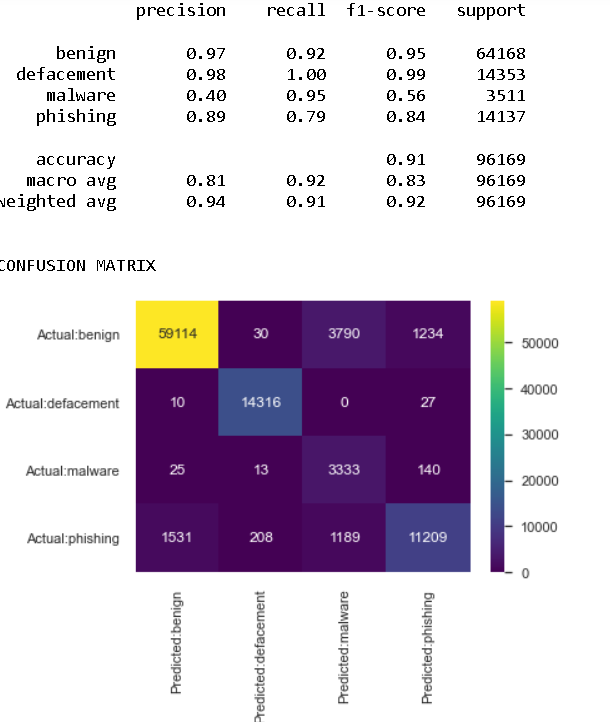
\includegraphics[width=1\textwidth]{RFclassification.png}}
\caption{Classification and confusion matrix report of Random Forest}
\label{Claaification Report of RF }
\end{figure}



In this project, we found that the Random Forest technique performed really well. It had high accuracy rates during both the training phase (99.9\%) and the testing phase (91.4\%). When examining the benign class, we calculated precision and recall scores of 92\% and 97\%, respectively.Foe more understanding we can refer to the\ref{Claaification Report of RF } the classification report and confusion matrix shown in the accompanying figure.

\subsection{Decision Tree:}


Decision trees (DT) are a method that is not parametric commonly used in supervised learning for the purposes of classification and regression. What exactly distinguishes them is their capacity to function efficiently with minimal pretreatment of data \cite{YANG201361}, in contrast to certain alternative classification methods that need procedures such as data normalisation, generation of dummy variables, or handling missing values. It is important to note that data transformers (DTs) do not possess an intrinsic capability to manage missing values. From a visual perspective, a decision tree (DT) can be metaphorically compared to a hierarchical structure resembling a tree, where the qualities are represented as nodes. A compelling recurrent pattern emerges during the process of classification.

\begin{figure}[htb]
\centering
\centerline{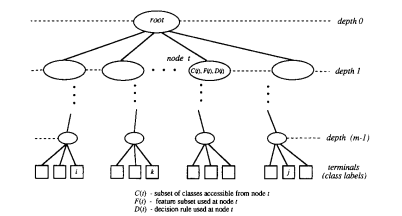
\includegraphics[width=1\textwidth]{DTexample.png}}
\caption{Example of Decision Tree Classifier}
\label{example DT }
\end{figure}

In essence, decision trees (DTs) consist of a collection of nodes originating from a single root node as shown in the above figure\ref{example DT }, with each of these nodes subsequently branching out into various directions. One intriguing characteristic of this particular structure is that the root node does not have any incoming edges, yet all succeeding nodes, also known as leaves \cite{YANG201361}, have precisely one incoming edge. As the classification process progresses, it is possible for these leaves to divide into sub-nodes under the guidance of the input training data. It is important to acknowledge that within every leaf node, there exists a probability vector that functions as an indicator of the likelihood associated with particular values of the target property.

The accuracies obtained for both the training and testing phases are 85\% each. The precision and recall scores for the "benign" category are significant, with values of 86\% and 95\% respectively. The comprehensive classification report and the confusion matrix for the decision trees model are displayed in Figure \ref{Classification and confusion matrix report of DT } for reference.

\begin{figure}[htb]
\centering
\centerline{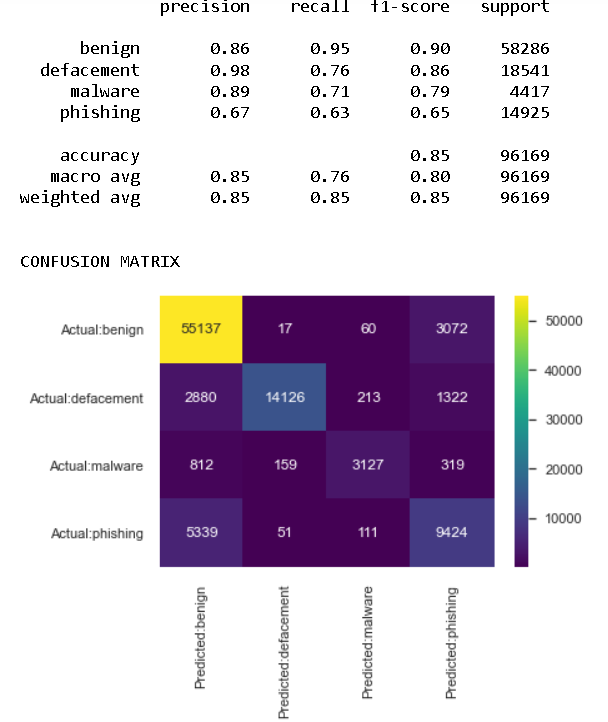
\includegraphics[width=1\textwidth]{DTclassification.png}}
\caption{Classification and confusion matrix report of Decision Tree}
\label{Classification and confusion matrix report of DT }
\end{figure}

\newpage
\section{Hyperparameter Tuning}



Parameters are crucial components of machine learning models, since they are responsible for their initialization and ongoing adjustment during the learning process. whereas,\cite{YANG201361} hyperparameters play a crucial role in determining the specific parameters that contribute to maximising the accuracy of the model. The hyperparameters can be manually specified or initialised by methods such as grid search cross-validation or randomised search cross-validation.

It is crucial to acknowledge that the determination of hyperparameters cannot be immediately inferred from the training data alone. However, it is imperative that these factors are determined prior to initiating the training process of a machine learning model. The hyperparameters play a crucial role in guiding the model to select the method that minimises the loss function. Consequently, the efficacy of machine learning algorithms can be significantly improved by engaging in the practise of fine-tuning, which entails the systematic examination of various parameter combinations.

Within the realm of machine learning algorithms, a wide range of parameters can be observed. The quantity and characteristics of these factors can vary considerably across different algorithms. The process of fine-tuning algorithms by modifying various parameters ultimately leads to the determination of the most optimal parameter configurations for any specific algorithm\cite{YANG201361}.


\newpage
\section{Cross Validation}



In a machine learning data science project, it is crucial to recognise the significance of each phase, starting from data collection to model deployment. The first step is to divide the dataset into two sets: the training set and the testing set. For this specific project, the data was divided into a training dataset of 70\% and a testing dataset of 30\%. The training dataset, which makes up 70\% of the data, is used to train the model. However, the remaining 30\% of the data, which is known as the test data, is used to evaluate the accuracy of the model.

The process of splitting data into training and testing subsets includes a random selection procedure. The randomness in this situation brings about uncertainty, which could result in cases where specific data in the testing set may not exist in the training set. As a result, this discrepancy can have a detrimental effect on the accuracy of the model. In order to tackle this concern, we can turn to the concept of K-fold cross-validation, which provides a more reliable way to assess prediction error.

In terms of computational efficiency,\cite{wong2019reliable} K-fold cross-validation is commonly preferred over leave-one-out cross-validation. The random state parameter used in the train-test split can be set to any numerical value. The selection of data points is determined by the choice of this random state number. When we change the random state number, it causes different sets of data points to be selected. This, in turn, leads to variations in the accuracy outcomes.

The K-fold cross-validation technique is introduced to reduce variability and improve accuracy assessment. Having a sufficient amount of training data is extremely important when it comes to constructing a dependable model. In K-fold cross-validation\cite{yadav2016analysis}, the dataset is split into training and testing subsets using a specific integer value called 'k.' Every value of 'k' represents a different experiment. In this example, we have a dataset with 10,000 records. We will be conducting five experiments, with 'k' set to 5.

For the first experiment, we use the first 2,000 records for training and keep the remaining 8,000 records for testing. In the following experiments, the model is trained using the next 2,000 records and then evaluated using the same set of 8,000 records. The purpose of this rotation is to ensure that the data points used for training in one experiment are used as the testing data in subsequent experiments. The iterative process will continue until all five experiments have been completed. The experiments produce five different accuracy values, and the final accuracy is determined by finding the average of these values.



\newpage
\section{Metrics for classifier evaluation:}
\subsection{Accuracy:}


The idea of accuracy is about determining the ratio of correct predictions to all the predictions made. Accuracy faces a difficulty when tackling classification tasks that have a noticeable imbalance among various classes. The problem becomes evident when one specific class has a significantly larger representation in the dataset. In situations like these, if we consistently predict the dominant class, it may lead to a high accuracy score. Regrettably, this demonstration does not effectively highlight the model's ability to accurately predict the minority class, which typically exhibits lower accuracy\cite{javaid2016deep}\cite{yacouby-axman-2020-probabilistic}.



Predictions are divided into four separate categories, namely True Positive (TP), False Positive (FP), True Negative (TN), and False Negative (FN). When a positive test result matches a positive prediction correctly, we call it a True Positive (TP). On the other hand, when a positive test result goes against a correct negative prediction, it is called a False Positive (FP). In the same way, when a negative test result aligns with an accurate negative prediction, it is referred to as a True Negative (TN). On the other hand, if a negative test result goes against a correct positive prediction, it is considered a False Negative (FN).

\subsection{Precision:}



Precision, also known as Positive Prediction Value, is a measure that evaluates the accuracy of positive predictions. The quantification of it is primarily determined by calculating the ratio of True Positives (TP) to the total number of instances that were predicted as positive. The main focus of this metric is to reduce errors, especially when it comes to accurately predicting positive labels\cite{javaid2016deep}\cite{yacouby-axman-2020-probabilistic}. The formula for precision can be expressed in the following manner:

\[
\text{Precision} = \frac{\text{True Positives}}{\text{True Positives} + \text{False Positives}}
\]





\subsection{Recall:}



Recall is the term used to describe the process by which the model derives information based on the genuine facts that are available. The term used to refer to the True Positive Rate (TPR) or sensitivity is also known as such. The reason for using this terminology is because the projected values are obtained as positive values, which aligns with the existing True Positives (TP) in the given scenario. One challenge that arises with recall is its tendency to classify all instances as positive cases, which can have a negative impact on the overall performance scores of the model. TPR, also known as True Positive Rate, is a measure that compares the number of True Positives to the total of True Positives and False Negatives\cite{javaid2016deep}\cite{yacouby-axman-2020-probabilistic}. The formula for recall is given as follows:

$$\text{Recall} = \frac{\text{True Positives}}{\text{True Positives} + \text{False Negatives}}$$


\subsection{F1 Score:}


The F1 score is considered the most preferred metric for demonstrating the performance of a model. The way it works is by comparing various systems and evaluating how effectively the model performs in comparison to them. The score is typically calculated based on the precision and recall values of the model. In situations where there are multi-class systems, the F1 score might not give completely satisfactory results because there is no true negative reference. The lack of true negatives is also applicable when measuring recall and precision\cite{yacouby-axman-2020-probabilistic}.

The F1 score is a metric that combines precision and recall in a balanced way. The metric scores obtained from evaluating classification models usually range from 0 to 1. A score of 1 suggests that the model's performance is commendable.

 $$ F1 = 2 \cdot \frac{precision \cdot recall}{precision + recall} $$

 \subsection{Confusion Matrix:}
 

The utilisation of a confusion matrix arises when there is a need to visually depict the degree of concordance between our predictive outcomes and the true categories. A representation of this matrix can be observed in Figure\ref{example CM }\cite{ARAVINDA20221}. Various assessment metrics can be derived from this matrix, encompassing recall, precision, and the F1 score, among others.

\begin{figure}[h]
\centering
\centerline{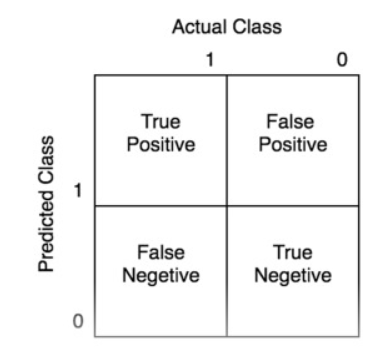
\includegraphics[width=1\textwidth]{confusionexample.png}}
\caption{Example of Confusion Matrix adopted from \cite{ARAVINDA20221}}
\label{example CM }
\end{figure}







\label{ch:2}

\setlinespacing{1.44}
%\bibliographystyle{agsm} % Use Harvard style 
\bibliographystyle{plain}
\bibliography{MyBib} % use your own bib file
\end{document}